%%%% CAPÍTULO 4 - RESULTADOS E DISCUSSÃO

\chapter{RESULTADOS E DISCUSSÃO}\label{cap:resultados}

De forma geral, o trabalho atingiu todos os objetivos estabelecidos. 
Desde a elaboração do \textit{hardware} para aquisição dos 
sinais, como também a implementação de um código otimizado e organizado (detalhado no 
\autoref{cap:apendicea}). Adicionalmente, 
a construção de uma interface gráfica e física, além da 
implementação de um módulo para cadastrar e excluir usuários.

\section{Protótipo \textit{hardware}}\label{sec:contrucaoprototipo}

Conforme pode ser observado na \autoref{fig:placapcb} 
o projeto da PCB (Placa de Circuito Impresso) foi construído 
com base no esquema elétrico da \autoref{fig:circuito}. 

\begin{figure}[h!]
    \centering
    \caption{Projeto da placa de circuito impresso do protótipo}
    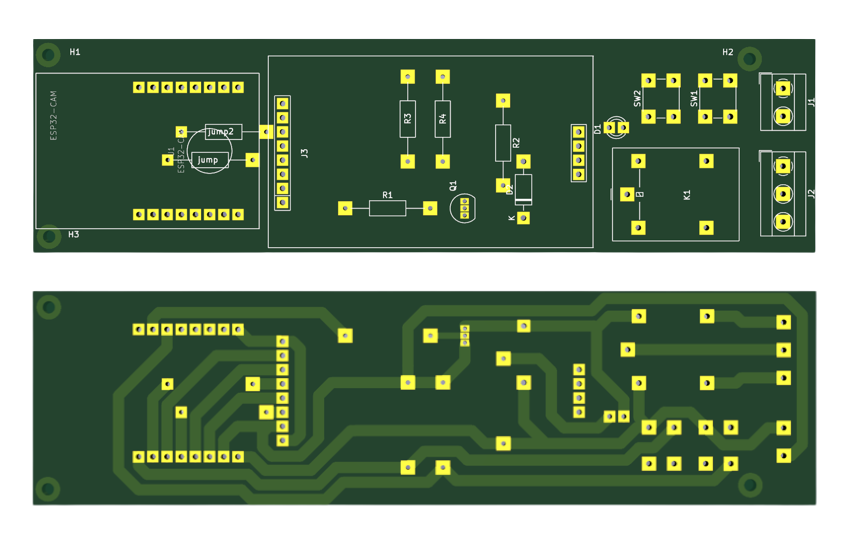
\includegraphics[scale=0.22]{figuras/placa_pcb.png}
    \fonte{}%% Fonte
    \label{fig:placapcb}
    \centering
\end{figure}

Após a conclusão da PCB foi feita a montagem 
da placa, como ilustrado na \autoref{fig:placamanufaturada}. 
Nela foi adicionada barras de pinos fêmea no lugar dos 
conectores do ESP32-CAM e do \textit{Display} TFT, para facilitar 
a remoção e a substituição desses componentes. Esse recurso 
é especialmente útil para o ESP32, permitindo a conexão com o 
gravador sempre que for necessário.

\begin{figure}[h!]
    \centering
    \caption{Placa manufaturada}
    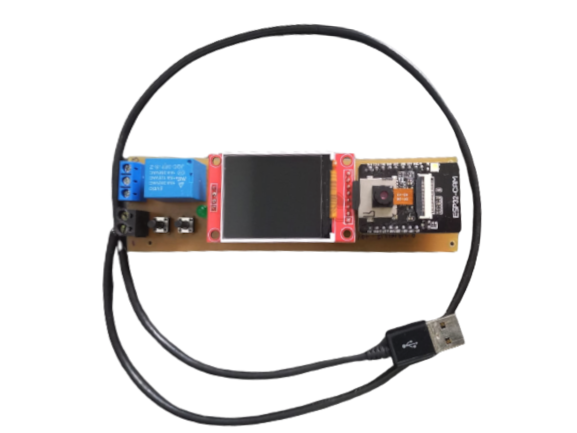
\includegraphics[scale=0.32]{figuras/placa_montada.png}
    \fonte{}%% Fonte
    \label{fig:placamanufaturada}
    \centering
\end{figure}

E assim que a placa foi confeccionada, projetou-se uma caixa para cumprir 
dois propósitos essenciais: proteger o circuito eletrônico e oferecer um 
acabamento esteticamente agradável para o usuário. Após a realização da 
modelagem 3D e da impressão, o protótipo da caixa 
foi acoplada à placa conforme ilustrada na \autoref{fig:placamontada}. 
Além de proteger o \textit{hardware}, a caixa contribuiu com uma apresentação 
mais amigável, melhorando a experiência de uso.

\begin{figure}[h!]
    \centering
    \caption{Placa montada}
    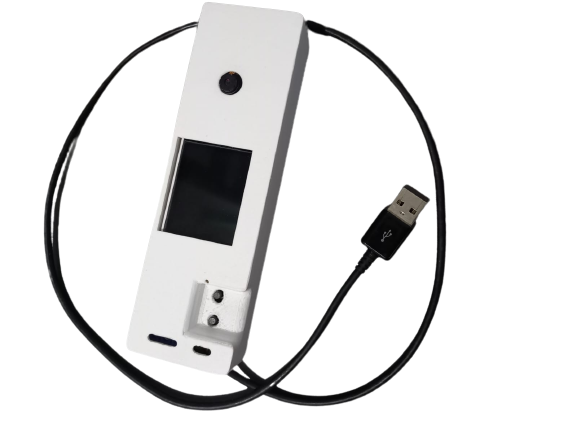
\includegraphics[scale=0.26]{placa_case.png}
    \fonte{}%% Fonte
    \label{fig:placamontada}
    \centering
\end{figure}

\section{Interface gráfica e física}\label{sec:interfacegrafica}

As interfaces gráficas foram elaboras para auxiliar os 
usuários na utilização protótipo. Desta forma, 
o primeiro conjunto de telas (\autoref{fig:fluxoinicial}) são referente à 
inicialização dos recursos utilizados no protótipo 
(câmera, sensores e o sistema de arquivos \textit{flash}).

\begin{figure}[h!]
    \centering
    \caption{Telas de inicialização}
    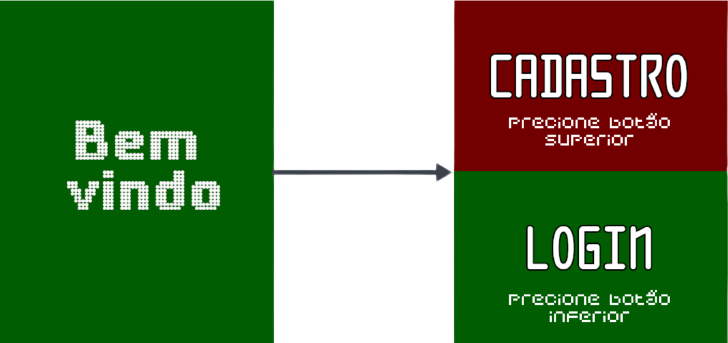
\includegraphics[scale=0.2]{figuras/fluxo_inicial.png}
    \fonte{}%% Fonte
    \label{fig:fluxoinicial}
    \centering
\end{figure}

Já as telas da \autoref{fig:fluxologin} 
correspondem ao fluxo do login, iniciando com a 
exibição de uma mensagem ao usuário,  em seguida a 
câmera é ligada para iniciar o processo de reconhecimento facial. 
Se o usuário estiver cadastrado, uma mensagem de sucesso é apresentada; 
no entanto, se não estiver, é exibida uma mensagem de erro.

\begin{figure}[h!]
    \centering
    \caption{Fluxo de telas do login}
    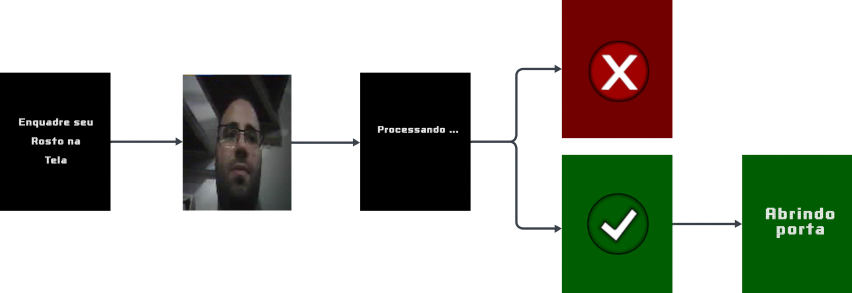
\includegraphics[scale=1.8]{figuras/fluxo_login.png}
    \fonte{}%% Fonte
    \label{fig:fluxologin}
    \centering
\end{figure}

Outro fluxo semelhante é o do cadastro, conforme ilustrado na \autoref{fig:fluxocadastro}.
Em contraste ao processo de login, a primeira tela solicita uma senha, e as telas 
subsequentes dependem do valor inserido pelo usuário. Se o usuário 
inserir corretamente a senha, a tela seguinte exibirá a mensagem 
''Senha correta'', seguida pela ativação da câmera para iniciar 
o processo de reconhecimento facial.
Após a conclusão do cadastro, os dados do reconhecimento são
armazenados na memória \textit{flash}, como indicado na \autoref{fig:dadosmemoria}, 
e uma mensagem de sucesso é exibida. No caso de algum erro, 
uma mensagem de erro é apresentada.

\begin{figure}[h!]
    \centering
    \caption{Fluxo de telas do cadastro}
    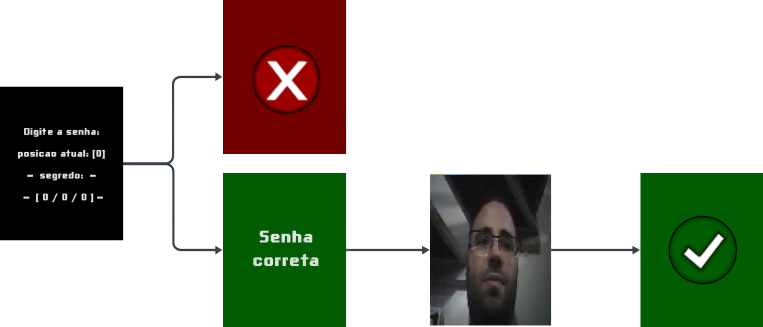
\includegraphics[scale=2]{figuras/fluxo_cadastro.png}
    \fonte{}%% Fonte
    \label{fig:fluxocadastro}
    \centering
\end{figure}

\begin{figure}[h!]
    \centering
    \caption{Lista de arquivos salvos na memória \textit{flash}}
    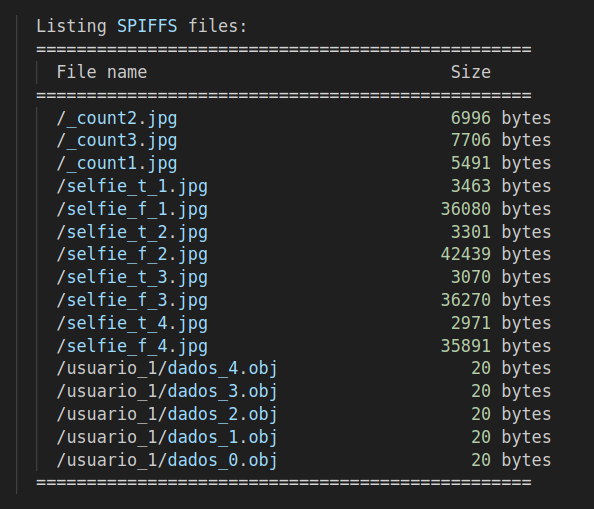
\includegraphics[scale=0.4]{figuras/dados_memoria.png}
    \fonte{}%% Fonte
    \label{fig:dadosmemoria}
    \centering
\end{figure}

O último fluxo é o processo de exclusão 
de usuários (\autoref{fig:fluxosenha}), que se assemelha 
ao fluxo do cadastro. Como pode ser observado, em ambos 
os casos, a primeira tela solicita a inserção 
de uma senha e o usuário tem aproximadamente 40 segundos 
digitar a senha correta. Durante esse tempo, 
pode ser exibida uma mensagem de ''usuários deletados'' ou 
exibido uma mensagem de erro. 

\begin{figure}[h!]
    \centering
    \caption{Fluxo de telas para deletar usuário}
    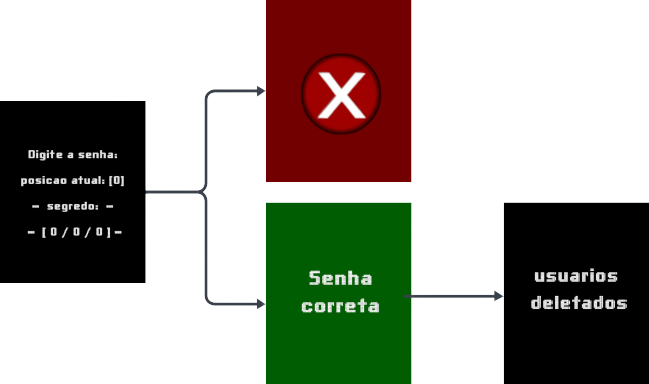
\includegraphics[scale=1.8]{figuras/fluxo_deletar_usuario.png}
    \fonte{}%% Fonte
    \label{fig:fluxosenha}
    \centering
\end{figure}

Dentre os fluxos já apresentados, aqueles que requerem 
senhas correspondem ao módulo do administrador, onde somente ele 
detém a capacidade de cadastrar ou excluir usuários. No decorrer 
desses fluxos, destaca-se a relevância da interface física 
(conforme ilustrado na \autoref{fig:botoesplaca}), 
composta pelos botões. Esses elementos possibilitam ao usuário a 
seleção tanto para acessar o login quanto para acessar o 
cadastro. Além disso, esses mesmos botões desempenham um 
papel importante para inserir os valores na tela de senha.

\begin{figure}[h!]
    \centering
    \caption{Interface física do protótipo}
    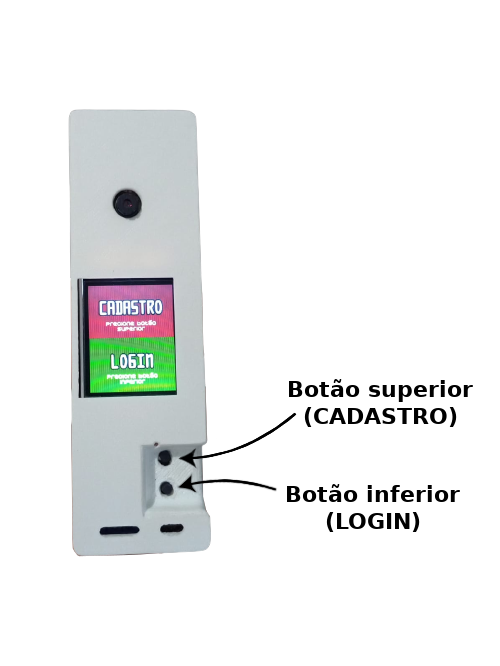
\includegraphics[scale=0.4]{figuras/placa_botoes.png}
    \fonte{}%% Fonte
    \label{fig:botoesplaca}
    \centering
\end{figure}

\section{Melhorias}\label{sec:melhorias}

Embora todos os objetivos estabelecidos tenham sido alcançados, 
ainda foi possível identificar algumas possibilidades para 
aprimorar o protótipo. Por exemplo, 
alterar o número máximo de usuários que podem se cadastrar. 
Também a inclusão de IDs para cada usuário, possibilitando a exclusão 
por meio desses identificadores. Outra consideração é permitir que 
o administrador altere as senhas associadas ao protótipo.

Uma melhoria interessante seria a ativação do módulo Wi-Fi, 
permitindo a integração do protótipo com aplicativos ou 
serviços web.

Por último, uma aprimoramento de grande impacto envolveria a 
criação de uma placa personalizada, inicialmente utilizando 
apenas o  \textit{chip} 
ESP32-S. Essa abordagem implicaria na liberação do I2C para 
uso geral, ampliando a disponibilidade de portas (GPIO) e 
possibilitando a incorporação de novos recursos.